\documentclass{article}

\usepackage{amsmath}
\usepackage{amsthm}
\usepackage{amssymb}
\usepackage{float}
\usepackage{graphicx}
\usepackage[utf8]{inputenc}
\usepackage[english]{babel}

\newtheorem{theorem}{Theorem}

\title{%
	Machine Learning: Collectives of local decision makers\\
	\large Formulating A Suitable Perceptron Paramaterisation
}
\author{Daniel Braithwaite}

\begin{document}

\maketitle

The goal of this project is to create neurons which insted of searching for a global minumum they will choose a specific part of the data to place their hyperplane. Consider the folowing situation in $\mathbb{R}^2$ where we have data split into two classes and the second class is boxed into a chevron shape. A single perceptron will go and place a horizonal line through the plane however this isnt telling us anything interesting. Prehaps something better to do is to align its self to one of the sides of the chevron, then if we added another "boundary hunter" it could align its self to the other side of the chevron.

\section{Simplified Situation}
Before worrying about this in the general case we aim to get a better understanding of the problem by first trying to solve the case described above. We first make some changes to how we have paramaterised our perceptron. We want to find a way which peforms the same as a standard perceptron before we start making it into a boundary hunter

\subsection{Point \& Gradient Paramaterisation}
We are trying to optimise a point (x,y) and a gradient. This is an alternative way to paramaterise our line. We are using sum squared error for our loss function and sigmoid as our activation. Each "boundary hunter" (BH) has the folowing weights vector $W = [m, x_0, y_0]$ and we consider two inputs to our BH, x and y. Our perceptron computes $z = (y - y_0) - m(x - x_0)$ and then outputs $o = f(z) = \frac{1}{1+e^{-z}}$.

\subsubsection{Deriving Gradients}
\begin{align}
\frac{\partial E}{\partial W_a} = \frac{\partial E}{\partial o} \frac{\partial o}{\partial z} \frac{\partial z}{\partial W_a}
\end{align}

\begin{align}
\frac{\partial o}{\partial z} = o(1 - o)
\end{align}

\begin{align}
\frac{\partial E}{\partial o} = -(t - o)
\end{align}

\begin{align}
\frac{\partial z}{\partial y_0} &= -1\\
\frac{\partial z}{\partial x_0} &= m\\
\frac{\partial z}{\partial m} &= x_0 - x
\end{align}

\subsubsection{Comparason To Perceptron}
If we use the same set of data to train both our standard perceptron and our modified perceptron we see that our modified dosnt quite peform as well as the standard version. For both models below they where trained for 50000 iterations of the training data.

\begin{figure}[H]
\centering
  \begin{minipage}[b]{0.4\textwidth}
    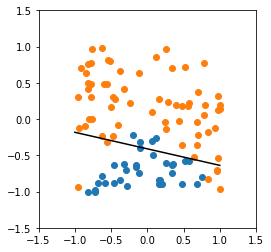
\includegraphics[width=\textwidth]{Standard-Perceptron.png}
    \caption{Standard Perceptron (SSE = 4.90)}
  \end{minipage}
  \hfill
  \begin{minipage}[b]{0.4\textwidth}
    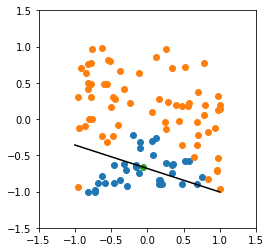
\includegraphics[width=\textwidth]{Modified-Perceptron-(Point-Grad).png}
    \caption{Modified Perceptron (SSE = 7.56)}
  \end{minipage}
\end{figure}

I propose that this way of constructing our perceptron is less powerful than the standard way. Consider when we are optimising our point-slope representation, 

\begin{align*}
y - y_0 &= m(x - x_0) \\
y &= y_0 + mx - mx_0 \\
y &= mx + (y_0 + mx_0)
\end{align*}

We have just shown that (as we would expect) we can convert out point-slope representation into a intercept-slope representation. From here we see we can convert into something that could be represented by our origonal perceptron.

\begin{align*}
y = mx + (y_0 + mx_0)\\
\Rightarrow -(y_0 + mx_0) -mx + y
\end{align*}

So given the generic form of our standard perceptron $A + Bx + Cy$ we see here that our modified perceptron can only ever learn a representation where C = 1, limiting what we can achieve. An easy way to check this is to see what happens if we use a standard perceptron to learn the data but keep the third weight (i.e. C) fixed at 1. Sure enough we get the folowing result when we run that experement over 50000 iterations.

\begin{figure}[H]
\centering
  \begin{minipage}[b]{0.4\textwidth}
    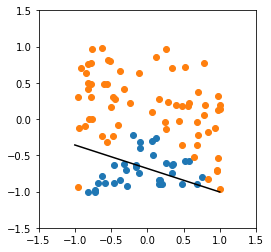
\includegraphics[width=\textwidth]{Standard-Perceptron-(C=1).png}
    \caption{Standard Perceptron with C = 1 (SSE = 7.56)}
  \end{minipage}
  \hfill
\end{figure}

So we are able to conclude that this method is unsuitable

\subsection{Normal \& Point Paramaterisation}
This method involves learning the normal vector (which is what the standard perceptron is doing) along with a point on the hyperplane. This increaes the number of paramaters we have to learn by n (when we are in $\mathbb{R}^n$ but this is necessary as to implement a BH we have to define some neighbourhood in which we care about and to do this we need to define it around some point on our hyperplane. So consider the folowing situation, we are learning the vector $n = [n_1, ..., n_n]$ normal to our hyperplane, the vector $a = [a_1, ..., a_n]$ which is on our hyperplane. We define $x = [x_1, ..., x_n]$ as our inputs making our weighted sum

\begin{align*}
z = \sum_{i=1}^n n_i * (a_i - x_i)
\end{align*}

We are still using SSE for loss and Sigmoid for actvation.

\subsubsection{Deriving Gradients}
\begin{align}
\frac{\partial E}{\partial W_a} = \frac{\partial E}{\partial o} \frac{\partial o}{\partial z} \frac{\partial z}{\partial W_a}
\end{align}

\begin{align}
\frac{\partial o}{\partial z} = o(1 - o)
\end{align}

\begin{align}
\frac{\partial E}{\partial o} = -(t - o)
\end{align}

\begin{align}
\frac{\partial z}{\partial a_i} &= n_i\\
\frac{\partial z}{\partial n_i} &= (a_i - x_i)\\
\end{align}

\subsubsection{Comparason To Perceptron}
Like before we compare the two paramaterisations using the same data and over 50000 iterations in the 2D case. In the graph for the modified perceptron the green point is our vector on the hyperplane.


\begin{figure}[H]
\centering
  \begin{minipage}[b]{0.4\textwidth}
    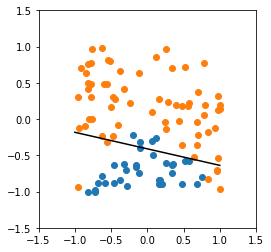
\includegraphics[width=\textwidth]{Standard-Perceptron.png}
    \caption{Standard Perceptron (SSE = 3.90)}
  \end{minipage}
  \hfill
  \begin{minipage}[b]{0.4\textwidth}
    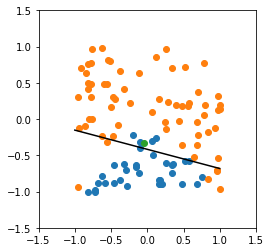
\includegraphics[width=\textwidth]{Modified-Perceptron-(Normal-Point).png}
    \caption{Modified Perceptron (SSE = 3.90)}
  \end{minipage}
\end{figure}

This modified perceptron has all the quallitys needed to proceid with creating the boundary hunters, whats better is this also generalizes to the $\mathbb{R}^n$ case.

\section{Boundary Hunter}
Using the \textbf{Normal \& Point Paramaterisation} from before we construct boundary hunters, first we have a simple case where the area of intererest for each boundary hunter is simpley a circle with fixed radius, our goal is to make this area of interest an ellipse which the BH will learn.

\subsection{Simplified Case}


\end{document}
